\documentclass[a4paper]{article}\usepackage[english]{babel}
\usepackage[utf8x]{inputenc}
\usepackage{amsmath}
\usepackage{graphicx}
\usepackage[colorinlistoftodos]{todonotes}
\usepackage[]{mcode}
\usepackage{placeins}
\title{Using a Lock-In amplifier to determine filters from High Pass, Low Pass and Band Pass circuits }
\author{Aaron Kebede}
\date{09/24/2021}
\begin{document}
\maketitle
\begin{abstract}
This report provides insight into the analysis of R-C Circuits. Hysteresis is defined as a retardation effect where the magnetisation of a magnetic material lags behind the magnetizing force. Here we will explore the hysteresis loop for a silver steel ferromagnet and use this to discover it’s magnetic properties. The method used will be to place a ferromagnet inside a solenoid with an alternating voltage which will continually reverse the magnetic field and magnetism direction. The relation between these two quantities will be used to produce a hysteresis loop from which magnetic properties can be deduced. 
The results obtained were: saturation magnetisation = $(8.4±0.5)(10^5)Am^{-1}$; remnant magnetisation = $(5.9±0.5)(10^5)Am^{-1}$; coercive field: $(4.3±0.5)(10^4)Am^{-1}$; energy expended per cycle per unit volume of material: $(1.55±0.05)(10^3)Jm^{-3}s^{-1}$; energy product: $(8.7±3.0)(10^4)Jm^{-3}$.

\end{abstract}

\section{Introduction}

Included in this report are details of the method, graphs, results, error analysis, discussions and conclusions of results.
Other researchers have found a lot in this area. As will be later referenced in the report, the values of the magnetic properties explored in this report have already been found to much more accuracy by other researchers.
The work here is related to the wider body of research however it does not provide any advancement in the field of ferromagnetism.
A practical application of ferromagnets is that they are used to make hard disks and credit cards. This is due to the ferromagnetic property of Hysteresis which provides magnetic memory in the material. Therefore memory is not erased which is very important in the items stated above.
A scientist named Alexander Stoletov was one of the first pioneer’s for electromagnetism. In 1871 he made the Stoletov curve showing magnetic permeability’s of ferromagnets. Since then, the area of science has gradually advanced and is now used widely.

\section{Theory}

The theory for this experiment is based around magnetic dipoles and solenoids. If we have a solenoid of ‘n’ turns and a current ‘I’ is passed through it, a magnetic field will be induced with a magnitude given in equation (1). Here $\mu_0=(4\pi)(10^{-7})Hm^{-1}$ is the vacuum permeability and ‘l’ is the length of the solenoid.

\begin{equation}\label{my_first_equation}
B= \frac{\mu_0nI}{l}
\end{equation}

The direction of this magnetic field is through the solenoid from end to end. This is in accordance with the right hand rule. If one was to curl the fingers of their right hand around the solenoid so that their fingertips pointed in the direction of current. Their thumb would point in the direction of induced magnetic field. Therefore, if we send a sinusoidally alternating current through a solenoid, the magnetic field will continually change direction by 180 degrees.
A silver steel ferromagnet contains dipoles pointing in random directions in the absence of a magnetic field. These dipoles are formed by the orbital directions of electrons. Figure [1] shows the magnetic field lines induced when and electron orbits. As can be seen, the magnetic field through the centre of the ring is vertically upwards.

\begin{figure}[!ht]
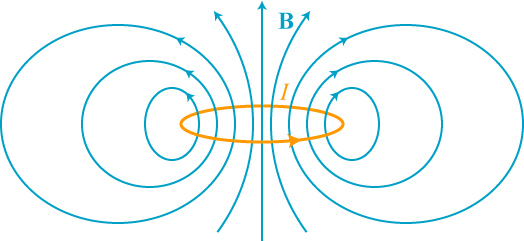
\includegraphics[width=\linewidth]{picture_1.jpg}
\caption{\label{fig:picture_1}Induced magnetic field 'B' lines caused by an electon’s orbit.}
\end{figure}

Adjacent electrons that have the same orbital direction have a net magnetic field pointing through the centre of each orbit according to the right hand rule. This net magnetic field is called a dipole. When an external field is applied from a solenoid, the electron orbits gradually align meaning the dipoles point in the same direction, thus forming a magnet. The act of the external field is to provide a torque (or moment) force on the electrons. Hence giving rise to the term ‘magnetic dipole moment’.
Magnetisation is defined as the vector field that represents the density of permanent or induced magnetic dipole moments in a magnetic material. Therefore, when an external magnetic field is applied, the magnetisation increases.
Ferromagnets have an interesting property called Hysteresis. When a ferromagnet is magnetised, it will not return back to zero magnetisation when the external field is removed. The field has to be reversed in order to decrease magnetisation back to zero. Therefore for ferromagnets, some energy must be expended in order to totally randomise the dipole’s directions once again after alignment. This is due to the fact that energy is required in order to generate an applied magnetic field. In the case of this experiment, the applied field was generated via a solenoid powered by the mains.
A vector which takes into account the alignment of the applied field ‘H’ and magnetisation ‘M’ is given the name: ‘magnetic flux density, ‘B’’. The equation relating these terms is given in equation (2):

\begin{equation}\label{my_second_equation}
B= \mu_0(H+M)
\end{equation}
If an alternating magnetic field is applied, a hysteresis loop is traced out with a graph of 'M’ against ‘H’. Figure (2) was sourced from reference (2). From this graph, and a graph of ‘B’ against ‘H’ (which is shown below in fig (3)), some magnetic properties of the ferromagnetic material used can be determined.

\begin{figure}[!ht]
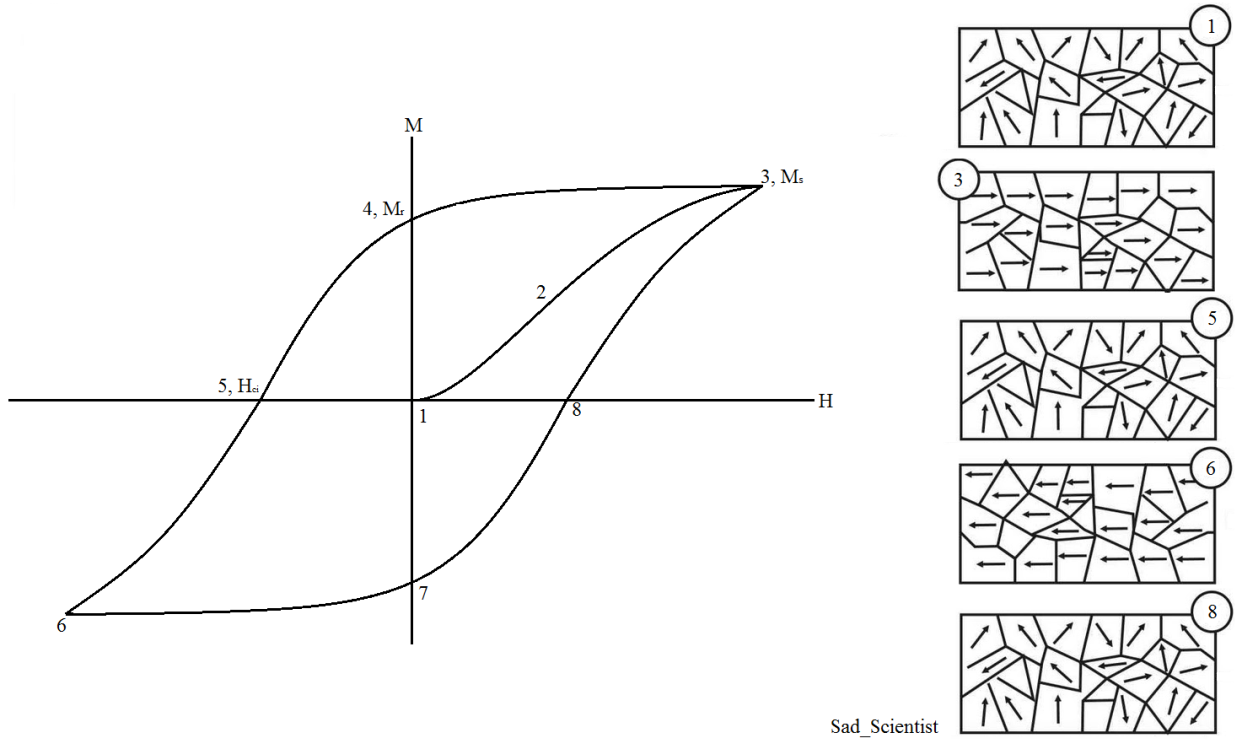
\includegraphics[width=\linewidth]{picture2.png}
\caption{\label{fig:picture2}Graph of magnetisation ‘M’ vs magnetic field inside sample ‘H’. The boxes on the RHS show the alignments of the dipoles at stages of the loop corresponding to the numbers on the graph. The dipoles are aligned the same way at maximum and minimum ‘M’, and are randomly arranged on the ‘H’ axis.}
\end{figure}

The values of ‘M’ at points 3 and 6 are equivalent to the positive and negative saturation magnetisation values. At these points, all of the dipole vectors are aligned in either the positive or negative direction, therefore these are the maximum and minimum possible magnetisation values.  The remnant magnetisation is the value of ‘M’ at point 4. This is the magnetisation that remains after the sample has had maximum positive applied field and now is under no applied field. Point 5 is equivalent to the coercive field. This is the modulus of the value of the magnetic field strength ‘H’ required to return the sample back to zero magnetisation.
From figure (3) some magnetic properties relating to the energy expended in the sample can be obtained. 

\begin{figure}[!h]
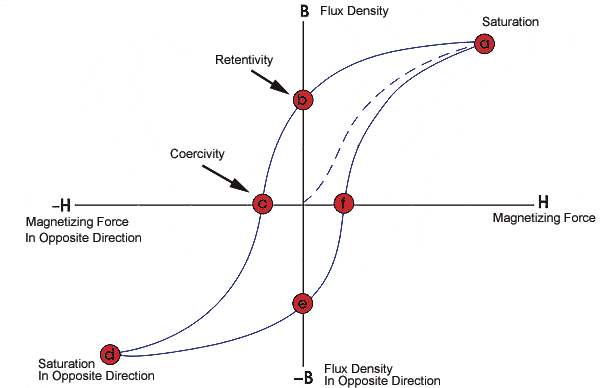
\includegraphics[width=\linewidth]{picture3.png}
\caption{\label{fig:picture3} Magnetic field inside sample ‘H’ vs magnetic flux density ‘B’ hysteresis loop. The dotted line indicates the initial path (at the start of the first sinusoidal cycle of applied magnetic field), the path then circulates anticlockwise around the bold line. }
\end{figure}
\FloatBarrier
As can be seen, the relation between ‘B’ and ‘H’ is not linear, instead a loop is made. The total area enclosed within the loop is equivalent to the energy expended during one cycle. Therefore, the greater the values of saturation magnetisation and coercive field, the greater the area of the loop, hence the more energy expended. Another measure of energy stored in the sample is the ‘energy product.’ As outlined in reference (4), the energy product is equivalent to the largest area of a rectangle drawn between the ‘B’ and ‘H’ axes with one of it’s corners on the loop. Energy product is commonly used for comparisons between different magnetic materials.
Harder ferromagnets have larger hysteresis loops, this is due to the fact that compared with soft ferromagnets, it takes more energy to change the dipole alignment. Therefore harder ferromagnets are used for permanent magnets whereas soft ferromagnets are used for temporary magnets.
A diagram for the experiment is shown below in figure (4):

\begin{figure}
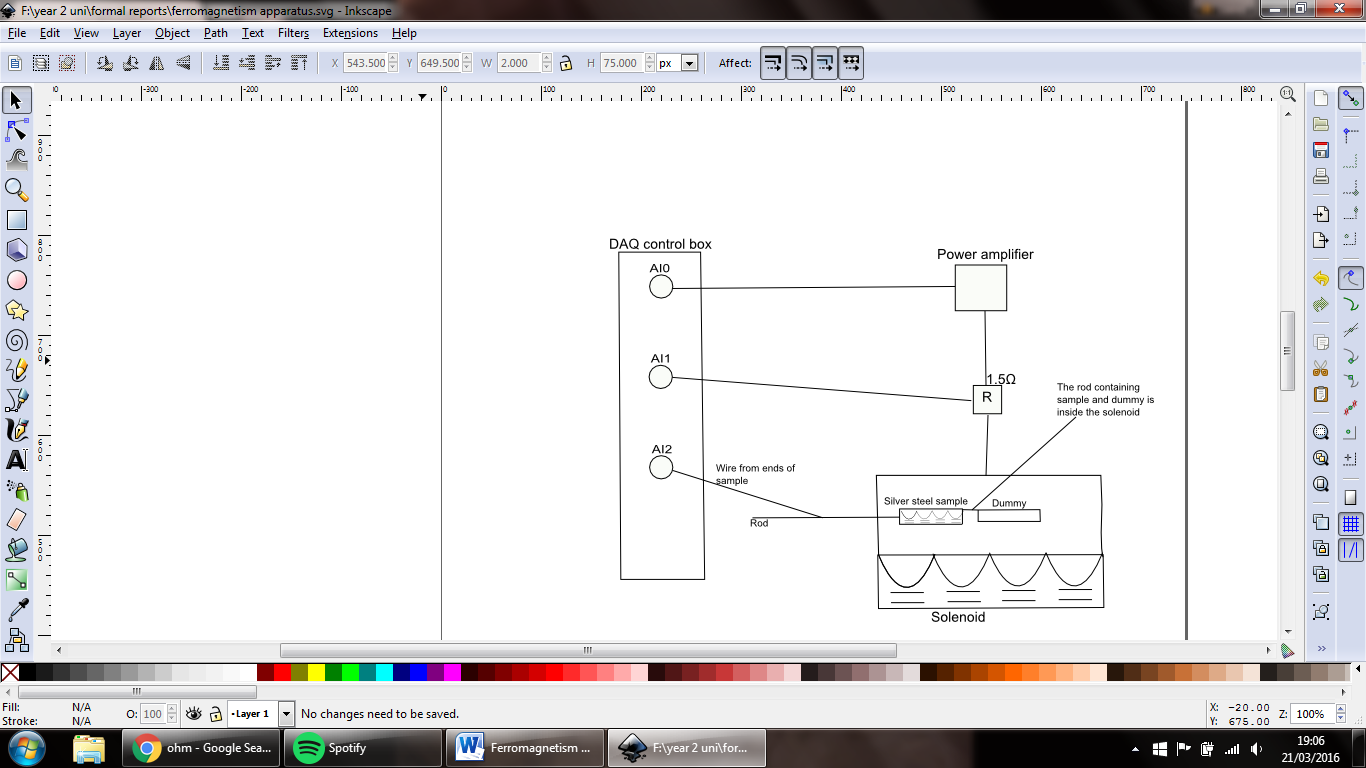
\includegraphics[trim=450 130 180 150,clip,width=10cm,clip,width=\linewidth]{picture4.png}
\caption{\label{fig:picture4}Diagram of the components of the experiment. }
\end{figure}
\FloatBarrier
A sinusoidal voltage can be supplied from the power amplifier via Matlab programming through the AI0 port. This alternating voltage can then be measured via the AI1 port and then dropped over the solenoid. An alternating current through a solenoid produces a magnetic field from Faraday's law shown algebraically below (where ‘V’ is the voltage across the solenoid, n is the number of turns around the solenoid, ‘$\phi$’ is the magnetic flux and ‘t’ is the time from when the voltage was applied):

\begin{equation}\label{my_third_equation}
V(t)= n\frac{d\phi}{dt}
\end{equation}

The magnetic flux ‘$\phi$’ here is equal to the magnetic flux density ‘B’ multiplied by the cross sectional area of the coil ‘A’. Substituting equation (2) for ‘B’ from above, we obtain the expression relating voltage to applied field ‘H’ and magnetisation ‘M’:

\begin{equation}\label{my_fourth_equation}
V(t)= nA\mu_0\frac{d(H+M)}{dt}
\end{equation}

In this experiment we want to measure the ‘M’ and ‘H’ fields separately of our ferromagnet inside our large solenoid. The ferromagnetic sample will have both ‘H’ and ‘M’ magnitudes due to the fact that it is a magnetic material. The alternating voltage causes the dipoles to change direction therefore changing the magnetisation.
Whereas, if we were to use a dummy sample of non-magnetic metal with a solenoid around it carrying alternating voltage, it would experience the ‘H’ field and not an ‘M’ field. This is due to the fact that the alternating magnetic field does not alter the directions of dipoles in a non-magnetic material.
The two samples are shown below: 

\begin{figure}
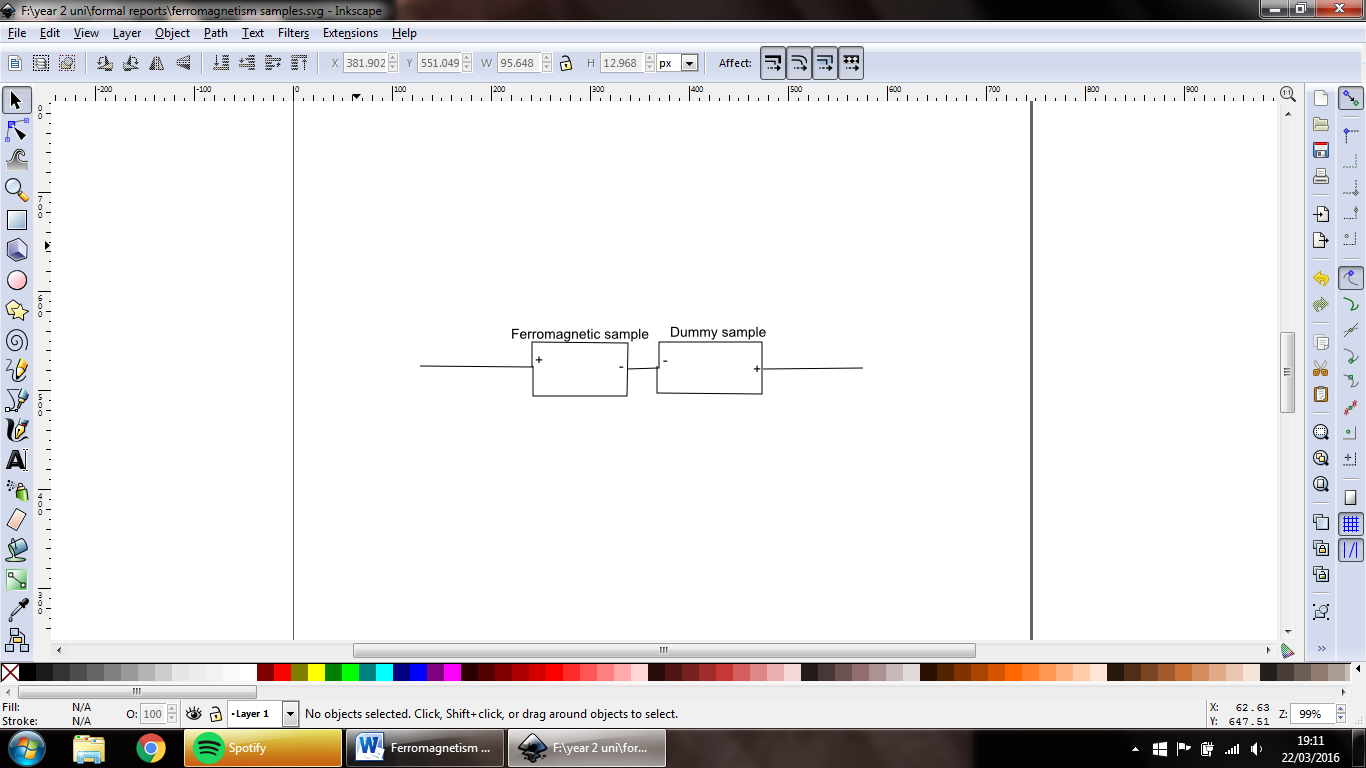
\includegraphics[trim=350 350 350 300,clip,width=10cm,clip,width=\linewidth]{picture5.png}
\caption{\label{fig:picture5}This shows the ferromagnet and dummy samples on the rod which is placed in the large solenoid. The ‘+’ and ‘-‘ signs denote positive and negative voltage.}
\end{figure}

The voltage across the ferromagnet sample is as in equation (4). Whereas, as there is no magnetisation in the dummy sample the voltage across it is shown below in equation (5):

\begin{equation}\label{my_fifth_equation}
V(t)= nA\mu_0\frac{dH}{dt}
\end{equation}

If we were to find the net voltage across both the ferromagnet and dummy sample we would be left with the following equation (6):

\begin{equation}\label{my_sixth_equation}
V(t)= nA\mu_0\frac{dM}{dt}
\end{equation}

Therefore, the magnetisation of the ferromagnetic sample can be obtained via manipulation of equation (6) to give equation (7):

\begin{equation}\label{my_seventh_equation}
M=\int_{0}^{t}\frac{V}{nA\mu_0}dt
\end{equation}

In Matlab, the function ‘cumtrapz(x,y)’ computes an approximation of the cumulative integral of ‘y’ with spacing ‘x’. The function ‘trapz(x,y)’ computes the integral of ‘y’ over ‘x’ increments. These functions can be used to integrate sample voltage over specific time spacing’s in order to produce an array of magnetisation.
We are now concerned with finding the magnetic field ‘H’ of the ferromagnetic sample. One might think this would be equivalent to the magnetic field of the large solenoid ‘$H_a$’, however we must take into account the demagnetising field. 
According to Maxwell’s equations, a condition of the magnetic flux density is that it must be continuous at boundaries between surfaces. A boundary condition for the demagnetising field ‘$H_d$’ is that it is discontinuous at surfaces with normal components of magnetism (at the ends of the ferromagnet). Therefore we can show the field lines of magnetic flux density, demagnetising field and magnetism below:

\begin{figure}
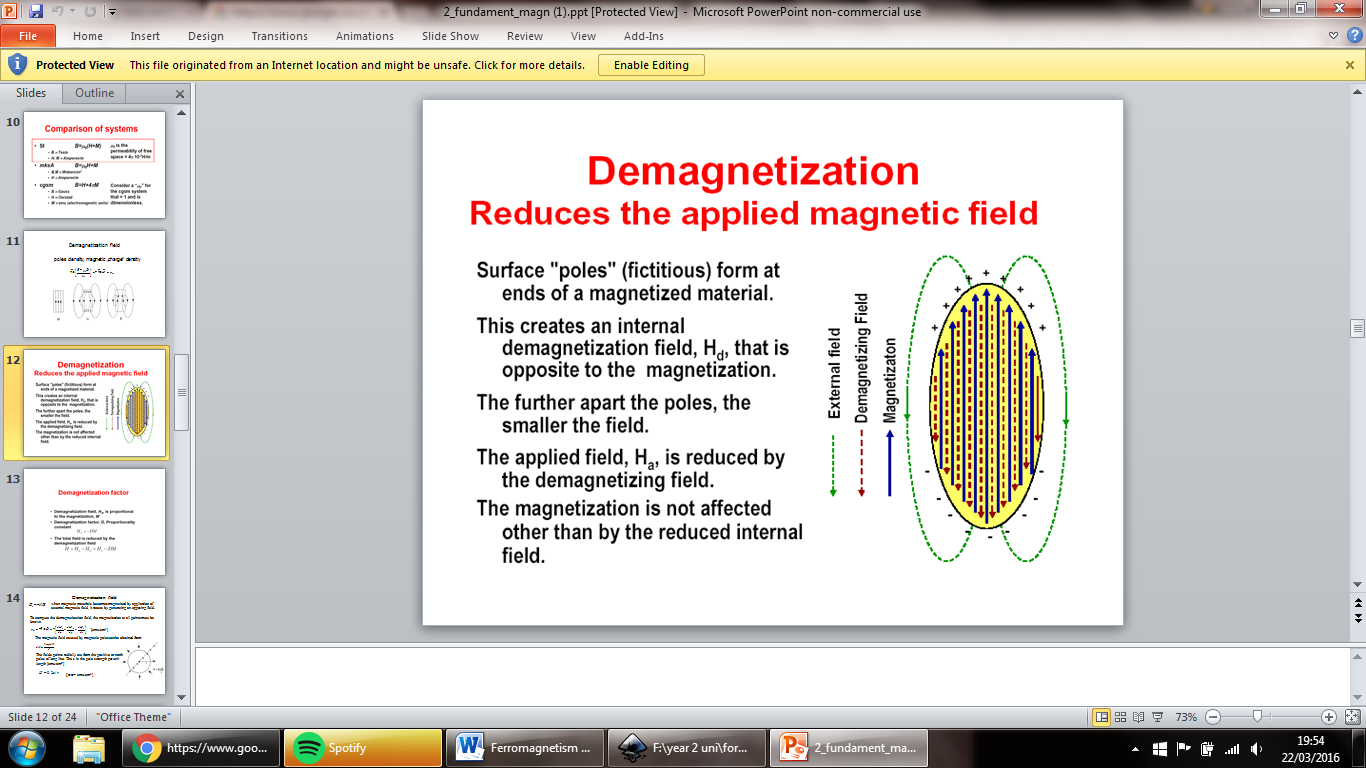
\includegraphics[trim=810 200 300 250,clip,width=10cm,clip,width=\linewidth]{picture6.png}
\caption{\label{fig:picture6}This shows the magnetic flux density (external field), the demagnetising field and the magnetisation of a ferromagnet.}
\end{figure}
\FloatBarrier
The direction of the demagnetising field inside the sample is such that it opposes the magnetic field which created it. Therefore the total magnetic field of the ferromagnetic sample is the sum of the applied and demagnetising fields. The demagnetising field is proportional to the magnetisation, therefore we can write this as a demagnetising factor ‘N’ multiplied by the magnetisation. This is expressed in equation (8) (where ‘$H_a$’ is the applied field and ‘H’ is the total field through the sample):

\begin{equation}\label{my_eighth_equation}
H=H_a-NM
\end{equation}

The demagnetising factor is given as a function of the aspect ratio which is shown in equation (9). Where ‘AR’ is the aspect ratio, ‘l’ is the length of the ferromagnet and ‘d’ is the diameter of the ferromagnet. Reference (5) explains this in more detail.

\begin{equation}\label{my_ninth_equation}
AR=\frac{d}{l}
\end{equation}

\section{Method}
First, the apparatus was set up as shown in figure (4) with the sample placed half way down the large solenoid. The reason why the position of half way down was chosen was because this was the part of the solenoid where the magnetic field was most uniform.
As shown in step (1) of the flow diagram in figure (7), a Matlab session was created and a sampling rate was chosen. I opted for a sampling rate of 1000 as this would produce many points on my graphs without the programme taking too long to run.
An array of time was then created and used to output a sinusoidal wave in series from the power amplifier to the resistor and to the large solenoid. The output wave had a frequency of 4Hz, a duration of one second and an amplitude of 5V. The 4Hz frequency was selected as this was low enough to allow the sample to saturate (to get to maximum or minimum magnetisation), yet high enough so that the sample was only just saturated before the magnetic field and dipoles began to change direction. The 5V voltage was chosen as this was the voltage where the hysteresis loops were shaped most similarly to that in figure (2).
Next, graph (1) from figure (8) (the caption explains how the graphs are numbered) was plotted of sample voltage against time. This produced a sinusoidal wave in the figure window of Matlab. After this, I removed the sample from the solenoid and ran the program to obtain another graph. What appeared was a noisy signal which wasn’t centred on zero volts. Therefore, in order to correct this systematic error, the mean of the noise was calculated using the ‘mean’ Matlab function. This mean was then taken away from the sample voltage array and replotted in order to obtain noise centred on zero volts. The sample was then placed back into the solenoid half way down.
After this, the values of ‘n’ and ‘A’ were needed for use with equation (7). The number of turns of the ferromagnet was 400. The diameter of the cylindrical ferromagnetic sample was found using a micrometer. Therefore the cross-sectional area was then found.
Next, the function ‘cumtrapz(t,V)’ was used to find the area between graph (1) and the ‘t’ axis. This was then used in equation (7) with the know values of ‘n’, ‘A’ and ‘$µ_0$’ to find the magnetism array for the ferromagnet. This was plotted (in graph (2)) against time. As was expected, the ‘M’ against  ‘t’ graph produced a minus-sine wave which was the integral of the minus-cosine graph from graph (1). 
Next, resistor voltage against time and power amplifier voltage against time were plotted in graphs (3) and (4) to give a greater understanding of how the experiment was working. After this, an array of current though the large solenoid was found. This was simply found considering Ohm’s law for a current in series through a resistor. The value of the resistor was noted on the resistor itself. This meant the graph of current against time (graph 5) was the factor of the resistor times less in vertical magnitude at every point.
Now the magnetic flux density inside the solenoid was plotted in graph (6). This was done using equation (1). A value of ‘n’ was written on the solenoid itself. The array of current was used as ‘I’. A larger micrometer was used to find the length of the ferromagnet ‘l’ than that used to find ‘d’.
After this, the magnetic field inside the sample was considered. We know from equation (8) that the demagnetising field has to be taken into account in order to find this. The aspect ratio was found and this allowed the demagnetising factor to be found using the graph in the lab manual. Therefore the magnetic field array could be computed from equation (8). This was then plotted against time in graph (7). 
Next the magnetic flux density of the sample was found using equation (2). Graphs (8) and (9) are hysteresis loops of magnetism against magnetic field and magnetic flux density against magnetic field. Now we are faced with the issue where we have four hysteresis loops and we only need one. To overcome this problem, the 80th to 305th elements of the magnetic field, magnetic flux density and magnetism arrays were reassigned to new variables in Matlab as these form one hysteresis loop instead of four. 
As can be seen from graphs (8) and (9) the hysteresis loops are not centred on the origin. This is an issue as it will produce systematic errors in results. Therefore, offsetting is required to re-centre these onto zero. This was done by taking the average of each of the three ‘B’, ‘H’ and ‘M’ arrays and taking this away from the arrays themselves. The new arrays were then used to make the ‘M’ against ‘H’ and ‘B’ against ‘H’ loops of graphs (10) and (11).
Now we have our desired hysteresis loops. We know from theory that the maximum ‘M’ value is the saturation magnetisation. The value of ‘M’ when H=0 is the remnant magnetisation, and the modulus of the value of ‘H’ when M=0 is the coercive field. We can look at our arrays and find the points of these arrays corresponding to the places mentioned and let these equal the saturation magnetisation, remnant magnetisation and coercive field values. 
Next, the magnetic flux density array was broken down into four parts corresponding to the four quadrants of the B vs H loop. The ‘trapz’ function was then used to find the areas of the four quadrants of graph (11). We were careful to use the transpose of the matrix if the matrix dimensions were not agreed in Matlab. These four area values were then added and the modulus taken. This value corresponded to the energy expended by the ferromagnet per cycle. However, we need to divide this value by the volume of the ferromagnet. This volume could be calculated (as the cross-sectional area and length were already known). Thus, we now have the energy expended per cycle per unit volume.
The energy product was found by visually looking at graph (11) and seeing where the largest box could be drawn in the second quadrant. The distances from this point to the origin along the horizontal and vertical axis were then found and then multiplied. This gave the area of the box which was equivalent to the energy product.


\usetikzlibrary{shapes.geometric, arrows}
\tikzstyle{process} = [rectangle, minimum width=3em, minimum height=2em, text centered, draw=blue, fill=gray!10]
\tikzstyle{startend} = [ellipse, minimum width=2em, minimum height=1em, text centered, draw=red, fill=gray!10]

\tikzstyle{arrow} = [thick,->,>=stealth]
\pagestyle{plain}
\begin{figure}
\centering
\hfill\\
{\scriptsize \begin{tikzpicture}[node distance=2em]

\node (S) [startend] {START};

\node (S1) [process, below of=S, yshift= -2em]{\parbox[t][][t]{10cm}{(1) create a session
}};
\draw [arrow] (S) -- (S1);
\node (S2) [process, below of=S1, yshift= -2em]{\parbox[t][][t]{10cm}{(2) Output a sinusoidal wave from power amplifier to resistor and solenoid
}};
\node (S3) [process, below of=S2, yshift= -2em]{\parbox[t][][t]{10cm}{(3) Plot sample voltage vs time
}};
\node (S4) [process, below of=S3, yshift= -2em]{\parbox[t][][t]{10cm}{(4) Calculate mean of noise and set zero offset
}};
\node (S5) [process, below of=S4, yshift= -2em]{\parbox[t][][t]{10cm}{(5) Integrate sample voltage and use this to plot M vs time ‘t’
}};
\node (S6) [process, below of=S5, yshift= -2em]{\parbox[t][][t]{10cm}{(6) Plot resistor voltage, power amplifier voltage, current and magnetic flux density all against t
}};
\node (S7) [process, below of=S6, yshift= -2em]{\parbox[t][][t]{10cm}{(7) Use demagnetising factor to plot magnetic field ‘H’ vs t for ferromagnet
}};
\node (S8) [process, below of=S7, yshift= -2em]{\parbox[t][][t]{10cm}{(8) Calculate magnetic flux density in the ferromagnet, then plot M vs H and B vs H hysteresis loops
}};
\node (S9) [process, below of=S8, yshift= -2em]{\parbox[t][][t]{10cm}{(9) Assign array corresponding to 1 loop, find offsets and centre loops on (0,0)
}};
\node (S10) [process, below of=S9, yshift= -2em]{\parbox[t][][t]{10cm}{(10) Plot M vs H and B vs H loops with the new arrays
}};
\node (S11) [process, below of=S10, yshift= -2em]{\parbox[t][][t]{10cm}{(11) Use arrays to find saturation magnetisation, remnant magnetisation, coercive field and energy product
}};
\node (S12) [process, below of=S11, yshift= -2em]{\parbox[t][][t]{10cm}{(12) Use trapz to find energy expended per cycle per unit volume
}};
\draw [arrow] (S1) -- (S2);
\draw [arrow] (S2) -- (S3);
\draw [arrow] (S3) -- (S4);
\draw [arrow] (S4) -- (S5);
\draw [arrow] (S5) -- (S6);
\draw [arrow] (S6) -- (S7);
\draw [arrow] (S7) -- (S8);
\draw [arrow] (S8) -- (S9);
\draw [arrow] (S9) -- (S10);
\draw [arrow] (S10) -- (S11);
\draw [arrow] (S11) -- (S12);
\node(S13)[startend, below of=S12,yshift=-2em]{STOP};
\draw [arrow] (S12) -- (S13);
\end{tikzpicture}}
\caption{\label{fig:picture7}Flow diagram showing the steps of my computer programming.}
\end{figure}

\section{Results}
The diameter of the ferromagnet was found using a micrometer to be (6.32±0.01)mm where the uncertainty was given as the precision of the micrometer. This corresponded to a cross-sectional area of $(3.14±0.01)(10^{-5})m^2$. Here the error was found considering error propagation. The equation used is shown in equation (10). Here the factor of ‘n’ is 2 because the diameter must be squared in order to obtain the area of a circle. ‘A’ is the cross-sectional area, ‘d’ is the circle diameter and the ‘∂’ represents the error in the quantity.

\begin{equation}\label{my_tenth_equation}
\frac{\delta a}{a}=2\frac{\delta d}{d}
\end{equation}

To obtain graph (5) the value of the resistor was required. This was written on the resistor itself to a precision of (0.1 $\Omega$) therefore this was taken to be the precision. Therefore resistance = (1.5±0.1)$\Omega$. 
The number of turns of the large solenoid was 2017 as this was written on the solenoid itself. The length of the ferromagnet was found with a different micrometer which only had a precision of ±0.1mm to be (152.5±0.1)mm. These values were used along with the array of current to obtain magnetic flux density against time in graph (6). 
Equation (9) was used in conjunction with the diameter and length of the ferromagnet along with the following error propagation equation in order to obtain an aspect ratio of (24.1±0.04). Here ‘AR’ is the aspect ratio, ‘l’ and ‘d’ are the length and diameter of the ferromagnet.

\begin{equation}\label{my_eleventh_equation}
\frac{\delta AR}{AR}=\sqrt[]{(\frac{\delta l}{l})^2+(\frac{\delta d}{d})^2}
\end{equation}
This corresponded to a demagnetising factor of (0.0037±0.0001) according to the precision of the graph supplied in the lab manual. This was used to define the array for the magnetic field of the ferromagnet plotted in graph (7). 
The cross-sectional area and length of the ferromagnet were multiplied together to find the volume of the ferromagnet. The value obtained was $(478±1)(10^{-8})m^3$. Here the error was obtained via the error propagation equation (11) as this equation is valid for both multiplication and division. Except ‘AR’ was replaced with volume ‘v’, and ‘d’ replaced with cross-sectional area ‘A’. The volume was needed in order to find the energy expended per cycle per unit volume.
The saturation magnetisation was found to be $(8.4±0.5)(10^5)Am^{-1}$, the remnant magnetisation: $(5.9±0.5)(10^5)Am^{-1}$ and the coercive force to be: $(4.3±0.5)(10^4)Am^{-1}$, the energy expended per cycle per unit volume to be: $(1.5±0.2)(10^3)Jm^{-3}s^{-1}$ and the energy product to be: $(8.7±3.0)(10^4)Jm^{-3}$. Here the errors were found considering error propagation and the standard deviation of repeats.








\begin{figure}
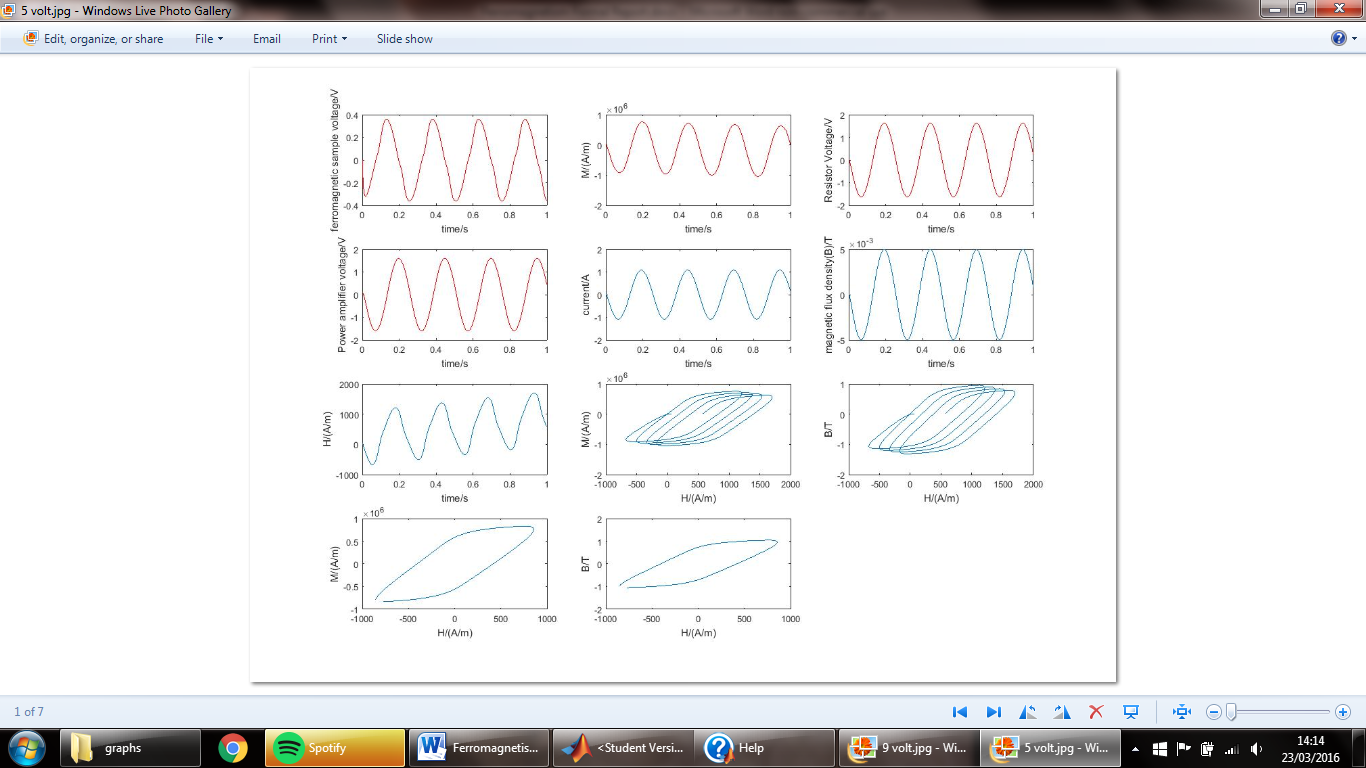
\includegraphics[trim=300 100 300 90,clip,width=10cm,clip,width=\linewidth]{picture8.png}
\caption{\label{fig:picture6}This figure shows the graphs created from my computer program. For referencing graphs in the text, the graph number will ascend across the page. Therefore graph (1) is the top-left, graph (2) is the top-middle, graph (4) is the 2nd row, 1st column etc.}
\end{figure}
\FloatBarrier
\section{Analysis}
The position of the ferromagnet down the large solenoid provided error. There was no way of knowing whether the ferromagnet was located at the centre of the solenoid. This was important as the centre was where the magnetic field was most uniform. Therefore random errors were made as a consequence of this. However this error was negligible in comparison to other errors.
There was some noise in the data from the sample voltage. This was indicated by the fact that the mean of the signal had to be computed with the ferromagnet not present in the large solenoid in order to correctly offset the data. This would therefore have provided a small source of random error throughout the experiment. 
The method used to find the saturation magnetisation was erroneous. As explained in the method, the peak magnetisation value for one run through of the experiment was taken to be at a certain place in the magnetisation array for all repeats of the experiment. However, the highest magnetisation value for a repeat may have occurred elsewhere in the array. This would have resulted in a magnetisation value being recorded which was not the highest. Therefore the true saturation magnetisation would have been missed. Similar is the case for the remnant magnetisation and coercive field measurements. Whereby, the correct value may have moved place in the array between repeats. Except in these cases, the value closest to zero of the magnetisation and magnetic field arrays was required, rather than the maximum value required for saturation magnetisation. Due to this source of error, a standard deviation value of $(±5(10^4))Am^{-1}$ was found. This was far greater than the error from propagation of precisions of instruments. This error was found on both the saturation magnetisation and remnant magnetisation values. The standard deviation on the coercive field was found to be $(±5(10^3))Am^{-1}$. 
The calculation of energy product had error associated with it due to the method used. As explained in the method, the sizes of the width and height of the box were chosen based on visually looking at the graph itself. There was therefore a high probability that a larger box could have been made corresponding to different sizes of width and height. Especially as the lengths of the magnetic flux density and magnetic field strength arrays for the single hysteresis loop were both 226. Due to the fact that this error had a far greater impact on the energy product than the precision of instruments, an error of $(±3(10^4))$ was found from standard deviation for the energy product. 
As can be seen in graphs (8) and (9), the hysteresis loops gradually shift to the right and slightly down with each new cycle. Theory suggests the loops should all lie on top of one another because the sample should magnetise and demagnetise by the same amount in each cycle.  The fact that all of the loops are almost exactly evenly spaced apart indicates systematic error. The reason behind the shift in loop position can be traced back to the sample voltage versus time graph (1). The voltage oscillates with the same positive amplitude and frequency. But the trough of the wave gradually moves down to a lower and lower voltage. The reason behind this is not known for sure but there are a few possibilities. One of which is that the chemical properties of the ferromagnet mean that it is magnetised better in one direction than the other. Another possibility is that the coils were not uniformly wrapped around the sample, meaning more magnetisation in one direction than the other. A faulty voltage signal from the power amplifier is not a possibility as graph (4) (the graph of power amplifier voltage versus time) shows a negative sine wave with no anomalies.
The micrometers used in this experiment seemed to function properly therefore the error on these can be assumed to be equivalent to their precision.

\section{Discussion}
The saturation magnetisation value from reference (6) was $(1.28±0.08)(10^6)Am^{-1}$. The value from this experiment was $(8.4±0.5)Am^{-1}$. The errors do not overlap and the percentage difference of 34\% indicates a fairly poor result. The major limiting factor here was the programming method in which the hysteresis loop was used to find the saturation magnetisation. A better method would have been to use the ‘max’ Matlab function to find the maximum magnetisation value in the array each time and use this as the saturation magnetisation.
The remnant magnetisation value from reference (6) was $(1.04±0.008)(10^6)Am^{-1}$.The value from this experiment was $(5.9±0.5)(10^5)Am^{-1}$. The errors do not overlap with the values and the percentage difference of 43\% indicates a reasonably poor experiment. As was the case with the saturation magnetisation, the key limiting factor here was the method of using the programming to obtain the value. Here, a better procedure would’ve been to find the modulus of the magnetic field array (by squaring and square rooting). Then using the ‘min’ function to find the lowest value in the array and using the magnetic field value corresponding to this value in the array. 
The coercive field value from reference (6) was $(5.3±0.1)(10^4)Am^{-1}$. The value obtained from this experiment was $(4.3±0.5)(10^4)Am^{-1}$. Therefore the errors do not overlap with the values but they are relatively close with a percentage difference of only 19\%. As was the case with the remnant magnetisation, the limiting factor was the method of programming and the way to improve the experiment would be to implement the same programming procedure as the one outlined for the remnant magnetisation. Except the magnetisation array should be manipulated instead of the magnetic field array. 
The energy product value from reference (6) was $(4.3±0.1)(10^4)Jm^{-3}$. The value obtained from experiment was $(8.7±3.0)(10^4)Jm^{-3}$. These values are quite far apart with a percentage difference of 102\% which should indicate a bad experiment. However, the error bars from the experiment nearly overlap the referenced value, therefore the experiment is almost scientifically viable. The main source of error in this value was in the method of finding the largest area of a box in the second quadrant of the hysteresis loop. This proved even more erroneous than the error in finding the saturation magnetisation, remnant magnetisation and coercive field. This is due to the fact that it was difficult to visualise where the largest box could be drawn (on graph (11)). A slight adjustment in the width or height of the box resulted in in a much larger change in the area of the box. This was due to the steep gradient of the hysteresis loop at the point where the box was placed in the second quadrant. A better way to compute this value would have been to set up a new Matlab array comprising of the product of the magnetic flux density and magnetic field. Then to find the maximum value of this array and to use this as the energy product.  
The energy expended per cycle per unit volume value from reference (6) was $(2±0.1)(10^3)Jm^{-3}s^{-1}$. The value obtained from this experiment was $(1.55±0.05)(10^3)Jm^{-3}s^{-1}$. Therefore the errors do not overlap but the values are fairly close. This is indicated by the percentage difference of 22\%. The error obtained has come from propagation of values used to obtain the hysteresis loop (such as aspect ratio and sample diameter) and the values used to obtain the volume of the ferromagnet (such as length and diameter). As can be seen the error is very small compared to the value itself. This indicates that systematic errors were more prevalent in this experiment than random ones. The errors arising from precisions of instruments were very small. This was due to micrometres having relatively good precision and the sampling rate of 1000 resulting in a very smooth hysteresis loop. The main source of systematic error is likely to have arisen from the four hysteresis loops not overlapping. Although this didn’t produce any measurable error (as the hysteresis loops remained the same shape) the fact that the loops were not aligned indicates that there was possibly something wrong with the ferromagnet sample or the way in which the wire was wrapped around it. There are no other obvious sources of systematic error. Therefore on the whole, the way in which this experiment could be improved so that the answers gained are closer to those referenced (in reference (6)) would be to closely examine the ferromagnet sample to see if there is fault with it. Then to find a way to resolve this problem and carry out an experiment which results in overlapping hysteresis loops and better results.

\section{Conclusion}
In conclusion, accurate results were very difficult to obtain from this experiment. The reason for this was the fact that the error analysis brought back the conclusion that the main source of error was systematic, and could logically only come from the ferromagnet itself. However, the experiment could have been vastly improved with more thorough programming procedures. This would have greatly reduced the errors on all of the results except for the energy expended per cycle per unit volume.
One good point was the shape of the hysteresis loops obtained. These were an almost exact replica of that shown in reference (2) and show that the theory was being realised in the experiment. One bad point was the misalignment of the hysteresis loops and the unclear nature of their presence. 
The values obtained by other researchers on the quantities examined are far more precise than those found in this experiment. Therefore the work in this project has not impacted the wider physical world.

\section{References}

1.	http://readingfeynman.org/2015/10/07/angular-momentum-in-quantum-\newline mechanics/\newline
2.	https://www.reddit.com/r/Elements/comments/l1ut9/magnetism\_and\_\newline magnets\_part\_4\_hysteresis/\newline
3.	https://www.nde-ed.org/EducationResources/CommunityCollege/\newline MagParticle/Physics/HysteresisLoop.htm \newline
4.	http://web.stevens.edu/e344/24\_fall\_2011/core/section\_7/FL\&O\_section\_7.\newline pdf (page 8)\newline
5.	http://www.jstor.org/stable/20022318?seq=1\#page\_scan\_tab\_contents\newline
 6.	http://www.kayelaby.npl.co.uk/general\_physics/2\_6/2\_6\_6.html

\section{Appendix}
Below is the Matlab code used in the investigation:
\setlength{\parindent}{0pt}
\setlength{\parskip}{18pt}
\begin{lstlisting}
clear, close all
daq.reset;

%Creating the session
s=daq.createSession('ni');
s.addAnalogOutputChannel('Dev1',0,'Voltage');
s.addAnalogInputChannel('Dev1',0:2,'Voltage');

%Setting sample rate
s.Rate=1000;

%setting frequency and duration of the signal.
freq=4;
duration=1;

%creating and plotting my sinusoidal input
time=(0:1/s.Rate:duration-1/s.Rate)';
voltage=5.*sin(2*pi*freq*time);
queueOutputData(s,voltage);

[data,timestamps]=startForeground(s);
figure(1)
subplot(4,3,1)

%Accounting for the offset of the data
offset=mean(data(:,1));
correctedv=(data(:,1))-offset;
plot(time,correctedv,'r-')
xlabel('time/s');
ylabel('ferromagnetic sample voltage/V')

%integrating voltage to find magnetisation
integral=cumtrapz(timestamps,correctedv');
m=(6.34e7).*integral;
subplot(4,3,2)
plot(timestamps,m,'r-')
xlabel('time/s');
ylabel('M/(A/m)')

%Plotting resistor voltage against time
subplot(4,3,3)
plot(time,data(:,2),'r-')
xlabel('time/s');
ylabel('Resistor Voltage/V')

%Plotting power amplifier voltage against time
subplot(4,3,4)
plot(time,data(:,3),'r-')
xlabel('time/s');
ylabel('Power amplifier voltage/V')

%Plotting current against time
current=(data(:,2))./1.5;
subplot(4,3,5)
plot(time,current)
xlabel('time/s');
ylabel('current/A')

%Plotting magnetic flux density against time
mu0=4.*pi.*(10.^-7);
n=2017;
l=0.553;
b=(mu0.*n.*current)./l;
subplot(4,3,6)
plot(time,b)
xlabel('time/s');
ylabel('magnetic flux density(B)/T')

%Plotting magnetic field strength against time
H=(b./mu0)-(0.0037*m');
subplot(4,3,7)
plot(time,H)
xlabel('time/s')
ylabel('H/(A/m)')

%Plotting M vs H hysteresis loops
subplot(4,3,8)
plot(H,m)
xlabel('H/(A/m)')
ylabel('M/(A/m)')

%Plotting B vs H hysteresis loops
subplot(4,3,9)
b_in=mu0.*(H+m');
plot(H,b_in)
xlabel('H/(A/m)')
ylabel('B/T')

%Getting arrays for one of the loops
loop4m=m(80:305);
loop4H=H(80:305);
loop4b_in=b_in(80:305);

%setting offsets for H,m and B
avloop4H=((max(loop4H))+min(loop4H))./2;
avloop4m=((max(loop4m))+min(loop4m))./2;
avloop4b_in=((max(loop4b_in))+min(loop4b_in))./2;

%reassigning values to centre them on the origin
betloop4H=loop4H-avloop4H;
betloop4m=loop4m-avloop4m;
betloop4b_in=loop4b_in-avloop4b_in;

%Plotting one hystersis loop of M vs H
subplot(4,3,10)
plot(betloop4H,betloop4m)
xlabel('H/(A/m)')
ylabel('M/(A/m)')

%Plotting one hystersis loop of B vs H
subplot(4,3,11)
plot(betloop4H,betloop4b_in)
xlabel('H/(A/m)')
ylabel('B/T')

%calculating saturation magnetisation
satmagpos=max(betloop4m)
satmagneg=min(betloop4m);

%calculating remanant magnetisation
remmag=betloop4m(153)

%calculating coercive field
coefie=betloop4H(181)

%calculating energy expended per cycle per unit volume
area1=(trapz(betloop4H(1:57)',betloop4b_in(1:57)'));
area2=(trapz(betloop4H(58:116)',betloop4b_in(58:116)'));
area3=(trapz(betloop4H(117:181)',betloop4b_in(117:181)'));
area4=(trapz(betloop4H(182:226)',betloop4b_in(182:226)'));
area=-(area1+area2+area3+area4)

%calculating energy product
bh=betloop4H(153:181).*betloop4b_in(153:181);
enprod=sqrt((min(bh)).^2)
 \end{lstlisting}

\end{document}